\documentclass{article}
\usepackage{graphicx}
\graphicspath{ {files/RCP_diagram/} {files/}}

\title{Multi-Scale Resolution of Human Social Systems:  A Synergistic Paradigm for Simulating Minds and Society}
\author{Mark G. Orr}

\begin{document}
\maketitle

\section{Introduction}
\cite{schelling1969}

Recently, we put forth an initial sketch of what we call the Resolution Thesis\cite{orr2018_brims}.  The thesis holds that 1) models of cognition will be improved given constraints from the structure and dynamics of the social systems in which they are supposed to be embedded, and 2) the resolution of social simulations of agents will be improved given constraints from cognitive first principles\footnote{Cognition considered as theoretical models of human perception, thought and action that includes, broadly, explanations of emotion, motivation, and affect in addition to more tradtional domains of cognitive psychology and cognitive science; in short, one could arguably use the term \textit{psychological first principles} as equivalent}.  This thesis reflects a variety of motivations, the most obvious being the observation that there is little overlap between the cognitive sciences and the generative social science approach[*REF EPSTEIN, 2008], both of which rely heavily on computer simulation to understand aspects of human systems, albeit different aspects of human systems with respect to scale.  The former focuses almost exclusively on the mind as a scientific object of study for which the lion's share of simulation efforts reflect a normative mind (one mind at a time, non-social or statically social) and the latter emphasizing multiple aspects of social systems, the mind being only one of these aspects, with the effect there is little cross-polination with the vast experimental evidence of how the mind operates or what are the central theoretical entities that compose the mind.  To a large degree, the resolution thesis is a recognition that the interdependence between cognitive and social systems has yet to be leveraged for the purposes of improving our understanding of both, despite some common points of interest.    

The Resolution Thesis can be understood from multiple perspectives.  From the view of cognitive science, the thesis means, broadly, that patterns of organization (e.g., information flow on the internet [REF; FROM SOCIALSIM], clustering of behaviors in a community[REF CHRISTAKIS] at the social and organizational level should inform the specifications of a cognitive model.  In other words, when possible, these patterns should be included as convergent evidence for a theory or model.  Naturally, it is desirable for cognitive models that are implicated in social behavior to have some reasonable explanatory scheme that links facets of the cognitive model to aspects of social organization.   We will address what this means and issues in more detail below but want to point the reader to Anderson's 200X Relevance Thesis as a useful example of reasoning about how cognition may have reasonable implications for social organization.   Furthermore, from the cognitive science perspective, neurophysiological processes are naturally implied and should be considered as a key part of the Resolution Thesis when appropriate [REF STOCCO here].  The reader might notice that it is difficult to think about using social organization as part and parcel of the convergent evidence of a cognitive model without considering the implications of cognition for social behavior.  But that is precisely the point--it is natural, once of the mind to think about how cognition scales, to think about using the degree to which it scales accurately as part of the convergent evidence for the validity of the model.


From the generative social science perspective, the Resolution Thesis means that the representations of agents should be informed closely by cognitive science and relevant neurophysiological considerations.  This runs somewhat counter to the principled adherence to simplification of the internal processing of simulated agents found in this literature, one that, in fact, served to show that complex social dynamics can be driven by simple behavioral rules of agents.  However, more recently, there are efforts in the generative social sciences that acknowledged that closer ties to the psychological and neurophysiological underpinnings of human behavior may yield benefit.  Epstein's neurocognitive approach is a notable effort in this vein[REF, Epstein 2014]; there are other related approaches (e.g. REF 19-22 from BRiMS).  These efforts notwithstanding, there remains a large gap between them and the implementation of models from cognitive science and psychology, not necessarily in principle, but in practice.  

A third and more general view is that the Resolution Thesis is about human systems for which the distinction between neural, cognitive and social levels of scale should be considered in unison.  An understanding of any of these levels of scale is dependent, to some degree, on an understanding of the others.  In effect, the notion of convergent evidence as originating, in part from other levels of scale, applies to all.  The implication is that we should leverage information from different levels of scale in an iterative and synergistic way, if not simultaneously [REF BRiMS paper][MAYBE REF ABDUCTION NAND 

The Resolution Thesis, despite sounding both reasonable and practical at face value, faces opposition from both the cognitive sciences and generative social sciences.  Simon's notion of nearly decomposable systems--that the temporal dynamics of adjacent levels of scale, in most systems, are little correlated--suggests that we can understand well the dynamics at each level of scale independently of the others(*REF, SIM 1962; see P. Anderson, 1972, for similiar argument in phyical systems).  The generative social sciences KISS (keep it simple, stupid) principle is clearly akin to Simon's notion, and is bolstered by the early wins in understanding the behavior of social systems (REF 15-17).   Another related, and possibley purer/stronger argument is that complexity arises in the midst of simplicity (e.g., May, 1976) a notion that is also well reflected in the origins of the generative social sciences (REF 15-17 from BRiMS).  In cognitive science, Newell, in considering the time scale of human behavior, suggested that the social band ($> 10^4$ seconds, representing social systems and organizational behavior) is characterized to be weak in strength in the sense that it may not provide computations in a systematic way (relative to lower temporal bands, e.g., cognitive and neural processes).  

These counter arguments notwithstanding, our working assumption is captured by the collquialism "The proof is in the pudding"  That is, the state of the art in technology, computing and the their tight coupling to the current social mileau affords, we think, the testing of the Resolution Thesis.   To this end, we've developed the \textit{Reciprocal Constraints Paradigm} (henceforth \textit{RCP}), to be discussed next.


\section{The Reciprocal Constraints Paradigm}
The \textit{RCP} is a methodological approach for thinking about how to develop understanding of social systems, and ultimately provide useable simulations of such.  It's value does not lie in precise presecription, but in laying a foundation for fruitful social simulation and an understanding of the implications for theory and models across levels of scale.  To be clear, the \textit{RCP} was conceived when considering multi-agent systems and cognitive science where human behavior, in both cases, is implemented in a simulation enviorment in which agents are represented algorithmically.  This is not meant to preclude other methods and approahces (e.g., analytically tractable economic games), but just to provide the context for the development of the ideas that underlie the \textit{RCP}.  We will address this concern in the discussion.

\begin{figure}
	\centering
	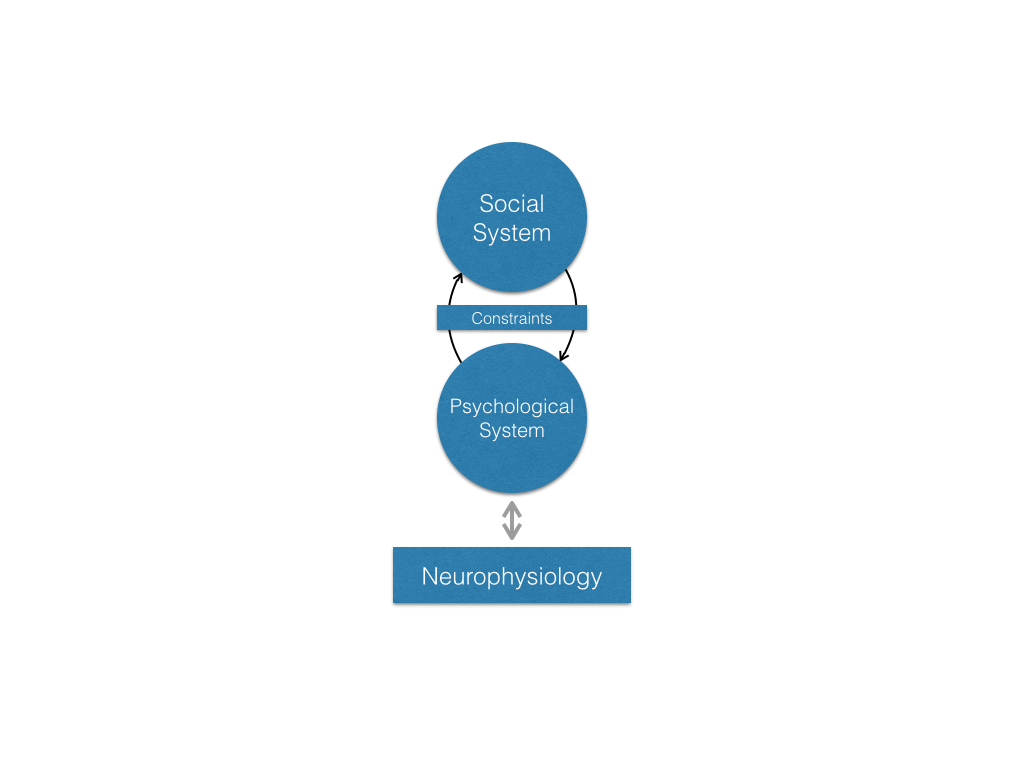
\includegraphics[width=1.0\textwidth]{RCP_diagram.png}
	\caption{\label{fig:rcpdiagram} The four  paradigm.  
	}
\end{figure}

Figure \ref{fig:rcpdiagram} shows the four primary components of the RCP: a cognitive system, an upward-scaling constraint, a social system, and a downward-scaling constraint.  Figure \ref{RCP_diagram} captures the potential for integrating neurophysiolgical considerations when appropriate; these may prove as essential for some social systems. Further, we assume that defining social systems and cognitive models as having an abstract set of first principles $S$ and $C$ and their implications (e.g., patterns expected in data and their interpretation); i.e., $S$ and $C$ are largely theoretical entities that determine properties of each level of scale (we expand on this shortly).  The upward- and downward-scaling constraints refers to using information from one level of scale to inform the resolution of another (we also expand on this shortly).  A fundamental component of constraints, as we see it, is that they are bound up in both theory and empirical/observation work in respect to the discipines that address a particular level of scale.  This makes defining what is $S$ and $C$ precisely more a matter of practice, at least in the initial stages of applications of the \textit{RCP}.



A central assumption in the RCP is that cognitive systems and definitions of agent behaviors in social systems are meant to represent human information-processing capacities that can be described as mathematical functions. \cite{van Rooij, 2008}\footnote{This is equivalent to Marr's computational level; we will use Marr's computational, algorithmic, and implementation levels of description\cite{Marr,1981} throughout this paper.}. Thus, in $C$ we can define a cognitive system as $\psi_{ct}: I_{ct} \rightarrow \psi_{ct}(i)$ where $I_{ct}$ is the set of allowable inputs and $\psi_{ct}(i)$ is the output; in $S$ we have a corresponding agent definition as $\phi_{at}: I_{at} \rightarrow \phi_{at}(i)$ where $I_{at}$ is the set of allowable inputs and $\phi_{at}(i)$ is the output for an agent\footnote{Social and cognitive systems may define parameters regarding variability among a set of agents; this is not reflected here.}.  Notice that $S$ and $C$ imply somthing about the inputs for both levels of scale as well as each's functional mapping.

The notion of reciprocal constraint in the \textit{RCP} reflects theorectical and empirical temporal and structural properties in $C$ and $S$.  A primary example in $C$ is the set of allowable algorithms $A$ such that $a \in C$ with grounding in empirical work in cognitive science and psychology.  This is a task complicated by the fact that within cognitive science and psychology there are sometimes strong disagreements concerning what is the right $A$, theroetically speaking, in terms of the task (what is the human analong that the models is representing).  Despite this difficulty, not all algorithms that compute $\phi_{at}$ are in $C$.  Primary examples in $S$ are the social structures, channels of information, and dynamics that characterize a social system, much of which is formalized using graph theory/network science.  These constraints in $S$ could directly affect the distribution of the inputs for a cognitive system.  It is important to emphasize that within $S$ are notions regarding the behavior of agents   


\subsection{Applying the Reciprocal Constraints Paradigm}   
In practice there are several approaches available for application of the RCT, but what unites them is the study of a human social phenomena, either defined at one level of scale or at multiple levels of scale.  Naturally, the first step is to identify a social phenonmena of interest, a task that is inherently tied to one's perspective.  If the perspective is largely in $C$, then the focus would most likely be on understanding the psychological processes, representations, etc. in relation to social systems; in other words a normative human\footnote{Individual differences do not preclude the notion of normative human but can be considered a parameter in such a theory}.   Another perspective, largely in $S$, would dictate a concern with the social structures and dynamics of the social system (multiple humans interacting) with some degree of constraint from $C$.  Of course, one could take the perspective that treats $C$ and $S$ simultanteously, which most likely depends on a simulation approach that captures aspects of $C$ and $S$ in one runnable system.  

\subsubsection{Single Scale Approaches}
It is conceivable that a fruitful applcation of the RCP might occur at one level of scale.  Let us first consider the cognitive level of scale.  There exists a large literature on neural and cognitive approaches to understanding human social behavior and social psychology\footnote{Division 8 of the American Psychological Association is dedicated to social psychology} with the requisite broad range of methods and theoretical orientations, so defining a social phenomena of interest is natural at the cognitive level. One potential approach, then, for implementing the \textit{RCP} would be to map key properties of cognitive systems to properties of social systems.  For example, one central finding in cognitive science and psychology is that learning mechanisms are sensitive to the order in which information is presented to the system (e.g., a human or computational model of a human).  Further, there is a large set of social phenomena that imply some type of learning mechanism (attitude formation [REF ORR]; impression formation [REF MONROE]).  Thus, we can conclude, reasonably, that order matters for some social phenomena at the psychological level.  The application of the RCT, in this case, means understanding inferring what a distribution of the temporal order of inputs would be given some $s \in S$ . (This distribution, almost axiomatically, seems dependent upon some propoerties of $S$ if $S$ contains graph $G$ where $V(G)$ and $E(G)$ are the agents and information channels, respectively.)  Off-hand, there seem to be candidate examples from the literature regarding human socio-technical networks(e.g., [REF BEARMAN; REF BARABASI WEB]), but what this means precisely would depend on the social phenomena of interest (e.g., early language development may depend on a different $G \in S$ compared to racial stereotypes).

At the social level of scale, an obvious approach is an analysis of the degree to which $\phi_{at}$ compares to any $\psi_{ct} in C$.  For the case in which $\phi_{at}$ and $\psi_{ct}$ are formally well defined, this might be relatively straigtforward\footnote{Potential methods for such a comparison would, idealy, focus not only comparison of input/output functions but also the strcuture of the runnable algorithm}.  But, there will certainly be cases for which this is not true.  For example, imagine that $\psi_{ct}$ is only defined in terms of an experimental paradigm, theoretical apparatus and the interpetation of data resulting from application of the experimental paradigm\footnote{Some might argue that under these conditions, the notion of a functional mapping $\psi_{ct}$ is nonsensical}.  One appraoch for comparison in this case would be to explore the behavior of $\phi_{at}$ by simulating an experimental paradigm that is isomphorphic to that used to define $\psi_{ct}$ (assuming $\phi_{at}$ is defined algorithmically).  In essence, this is like running an psychological experiment on artificial agents, an approach that is akin to simulation in the psychological sciences.  The output of these experiments could be compared to patterning and dynamics of human performance in $C$. To make this approach more concrete, consider agent definitions in generative social science invoke a threshold rule [REF ORR; a po]. 

The single scale approach, although useful, will always have the feature of missing potential important dynamics and structures at adjacent levels of scale. 
 

\subsubsection{Multi-Scale Approach}
to build a simulation platform that simultaneosly captures essentail aspects of both $S$ and $C$ (e.g., an agent-based model of cognitive agents) and to simulate a social phenomena.  In this case, the upward-constraints refer directly to the substition of  $\psi_{ct}$ for $\phi_{at}$; the downward-constraints refer to the degree to which the simulated social system matches $S$ as defined by the pheonomena of interest.  The downward constraints would thus serve as a signal that would suggest modifications to $\psi_{ct}$.  In this case $\phi_{at}$ is respected by the construction of the social simulation environment.

FREE PARAMETER PROBLEM AND Acountable modeling:  The second kind is to abstract some details from full-fledged cognitive models, but adhere to a principle of \textit{Accountable Modeling}\ref{LebiereX}.

 
The notion of generating a fixed system of constraints that can automate the construction of social systems.  $S$ and $C$ can be encoded as algorithms.  If this is the case, then we could construct an automated system that scans the parameter space (if computable).

What if $S$ is dependent on $C$?



\section{Analysis of Related Work}
Here we provide examples of prior work that employ parts of the RCP.  As we have no known examples of the downward-constraints, we focus on upward-constraints.  These are not exhaustive; we apologize for any work not mentioned.  

\section{An Example of RCT Implemented}
Christian's sim

Note, we may just provide examples of how Stocco's work might be used in our example...not run the actual sims if not have time.

\section{Discussion}
\subsection{Computational Complexity}
Both levels of scale should restrict to functions that are computable in polynomial time.  

\subsection{What Level of Scale for Initiation}
We advocate starting with the cognitive level in principle.  This might mean starting with a social system, implemented on a graph. 

\subsection{Social System Only and Graphical Dynamical Systesm}
There 

\subsection{Statistical and Analytical Models of Social Systems}
Can we apply the RCP to Statistical or Analytic models that do not have implementations in simulation environments?  Is this possible?  If yes, then what are the considerations?

\subsection{Importing Neurophysiology}
Provide background on Stocco's work.

\subsection{Issues \& Moving Forward}
From the single level of scale approach, One idea is to catalog social phenomena captured by psychological models and do a mapping of $C$ to $S$. \footnote{In the limit, the social features and the cognitive features have co-evolved on an evolutionary time scale}.

Issues of the right cogntive model, lots of cog models....

It should be clear that application of the RCP to social systems relies, in the end, of simulation approaches both at the cognitive and social levels.  Without this, the approaches are generally one level.  Even one level approaches that are formal and have sim, will still not capture the dynamics at play without full simualtion.  

%FIGURES



\bibliographystyle{plain}
\bibliography{references}

\end{document}